% Created by tikzDevice version 0.12.3.1 on 2022-01-05 18:46:22
% !TEX encoding = UTF-8 Unicode
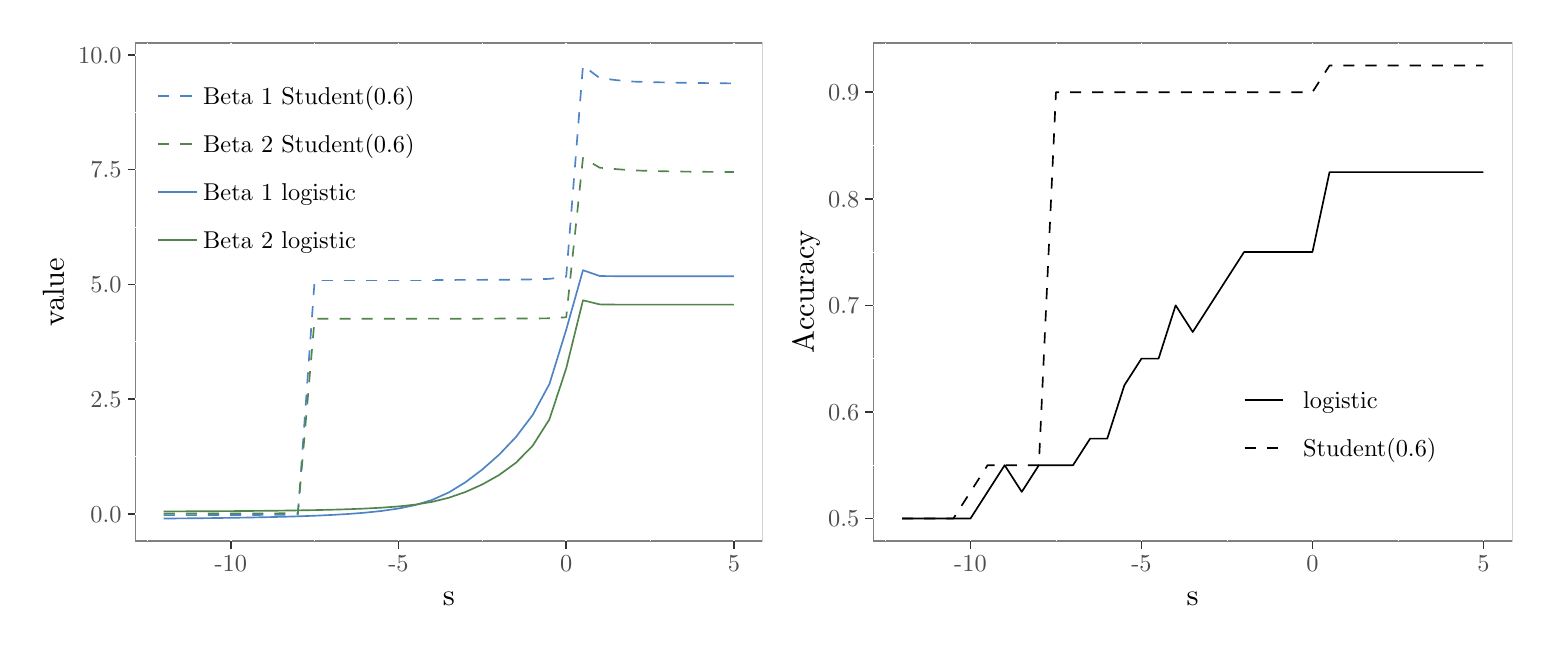
\begin{tikzpicture}[x=1pt,y=1pt]
\definecolor{fillColor}{RGB}{255,255,255}
\path[use as bounding box,fill=fillColor,fill opacity=0.00] (0,0) rectangle (542.02,216.81);
\begin{scope}
\path[clip] (  0.00,  0.00) rectangle (271.01,216.81);
\definecolor{drawColor}{RGB}{255,255,255}
\definecolor{fillColor}{RGB}{255,255,255}

\path[draw=drawColor,line width= 0.6pt,line join=round,line cap=round,fill=fillColor] (  0.00,  0.00) rectangle (271.01,216.81);
\end{scope}
\begin{scope}
\path[clip] ( 38.85, 31.25) rectangle (265.51,211.31);
\definecolor{drawColor}{gray}{0.50}
\definecolor{fillColor}{RGB}{255,255,255}

\path[draw=drawColor,line width= 0.6pt,line join=round,line cap=round,fill=fillColor] ( 38.85, 31.25) rectangle (265.51,211.31);
\definecolor{drawColor}{RGB}{255,255,255}

\path[draw=drawColor,line width= 0.3pt,line join=round] ( 38.85, 61.77) --
	(265.51, 61.77);

\path[draw=drawColor,line width= 0.3pt,line join=round] ( 38.85,103.27) --
	(265.51,103.27);

\path[draw=drawColor,line width= 0.3pt,line join=round] ( 38.85,144.77) --
	(265.51,144.77);

\path[draw=drawColor,line width= 0.3pt,line join=round] ( 38.85,186.27) --
	(265.51,186.27);

\path[draw=drawColor,line width= 0.3pt,line join=round] ( 43.09, 31.25) --
	( 43.09,211.31);

\path[draw=drawColor,line width= 0.3pt,line join=round] (103.69, 31.25) --
	(103.69,211.31);

\path[draw=drawColor,line width= 0.3pt,line join=round] (164.30, 31.25) --
	(164.30,211.31);

\path[draw=drawColor,line width= 0.3pt,line join=round] (224.91, 31.25) --
	(224.91,211.31);

\path[draw=drawColor,line width= 0.6pt,line join=round] ( 38.85, 41.02) --
	(265.51, 41.02);

\path[draw=drawColor,line width= 0.6pt,line join=round] ( 38.85, 82.52) --
	(265.51, 82.52);

\path[draw=drawColor,line width= 0.6pt,line join=round] ( 38.85,124.02) --
	(265.51,124.02);

\path[draw=drawColor,line width= 0.6pt,line join=round] ( 38.85,165.52) --
	(265.51,165.52);

\path[draw=drawColor,line width= 0.6pt,line join=round] ( 38.85,207.02) --
	(265.51,207.02);

\path[draw=drawColor,line width= 0.6pt,line join=round] ( 73.39, 31.25) --
	( 73.39,211.31);

\path[draw=drawColor,line width= 0.6pt,line join=round] (134.00, 31.25) --
	(134.00,211.31);

\path[draw=drawColor,line width= 0.6pt,line join=round] (194.60, 31.25) --
	(194.60,211.31);

\path[draw=drawColor,line width= 0.6pt,line join=round] (255.21, 31.25) --
	(255.21,211.31);
\definecolor{drawColor}{RGB}{78,132,196}

\path[draw=drawColor,line width= 0.6pt,dash pattern=on 4pt off 4pt ,line join=round] ( 49.15, 40.66) --
	( 55.21, 40.67) --
	( 61.27, 40.68) --
	( 67.33, 40.69) --
	( 73.39, 40.70) --
	( 79.45, 40.72) --
	( 85.51, 40.75) --
	( 91.57, 40.79) --
	( 97.63, 40.85) --
	(103.69,125.59) --
	(109.75,125.60) --
	(115.82,125.60) --
	(121.88,125.61) --
	(127.94,125.61) --
	(134.00,125.62) --
	(140.06,125.62) --
	(146.12,125.63) --
	(152.18,125.65) --
	(158.24,125.67) --
	(164.30,125.69) --
	(170.36,125.71) --
	(176.42,125.76) --
	(182.48,125.85) --
	(188.54,126.04) --
	(194.60,126.84) --
	(200.66,203.13) --
	(206.72,198.58) --
	(212.79,197.84) --
	(218.85,197.32) --
	(224.91,197.14) --
	(230.97,197.00) --
	(237.03,196.89) --
	(243.09,196.81) --
	(249.15,196.73) --
	(255.21,196.67);
\definecolor{drawColor}{RGB}{82,133,76}

\path[draw=drawColor,line width= 0.6pt,dash pattern=on 4pt off 4pt ,line join=round] ( 49.15, 41.27) --
	( 55.21, 41.27) --
	( 61.27, 41.27) --
	( 67.33, 41.28) --
	( 73.39, 41.29) --
	( 79.45, 41.29) --
	( 85.51, 41.30) --
	( 91.57, 41.32) --
	( 97.63, 41.35) --
	(103.69,111.62) --
	(109.75,111.65) --
	(115.82,111.63) --
	(121.88,111.64) --
	(127.94,111.62) --
	(134.00,111.63) --
	(140.06,111.65) --
	(146.12,111.67) --
	(152.18,111.63) --
	(158.24,111.64) --
	(164.30,111.66) --
	(170.36,111.69) --
	(176.42,111.72) --
	(182.48,111.71) --
	(188.54,111.79) --
	(194.60,112.16) --
	(200.66,169.75) --
	(206.72,166.20) --
	(212.79,165.69) --
	(218.85,165.23) --
	(224.91,165.04) --
	(230.97,164.90) --
	(237.03,164.80) --
	(243.09,164.73) --
	(249.15,164.69) --
	(255.21,164.65);
\definecolor{drawColor}{RGB}{78,132,196}

\path[draw=drawColor,line width= 0.6pt,line join=round] ( 49.15, 39.44) --
	( 55.21, 39.49) --
	( 61.27, 39.54) --
	( 67.33, 39.61) --
	( 73.39, 39.70) --
	( 79.45, 39.79) --
	( 85.51, 39.91) --
	( 91.57, 40.05) --
	( 97.63, 40.23) --
	(103.69, 40.45) --
	(109.75, 40.73) --
	(115.82, 41.08) --
	(121.88, 41.55) --
	(127.94, 42.18) --
	(134.00, 43.05) --
	(140.06, 44.30) --
	(146.12, 46.15) --
	(152.18, 48.87) --
	(158.24, 52.59) --
	(164.30, 57.17) --
	(170.36, 62.52) --
	(176.42, 68.87) --
	(182.48, 76.85) --
	(188.54, 88.07) --
	(194.60,107.67) --
	(200.66,129.17) --
	(206.72,127.07) --
	(212.79,127.00) --
	(218.85,127.00) --
	(224.91,127.00) --
	(230.97,127.00) --
	(237.03,127.00) --
	(243.09,127.00) --
	(249.15,127.00) --
	(255.21,127.00);
\definecolor{drawColor}{RGB}{82,133,76}

\path[draw=drawColor,line width= 0.6pt,line join=round] ( 49.15, 42.01) --
	( 55.21, 42.03) --
	( 61.27, 42.06) --
	( 67.33, 42.09) --
	( 73.39, 42.12) --
	( 79.45, 42.17) --
	( 85.51, 42.22) --
	( 91.57, 42.29) --
	( 97.63, 42.38) --
	(103.69, 42.48) --
	(109.75, 42.62) --
	(115.82, 42.80) --
	(121.88, 43.04) --
	(127.94, 43.36) --
	(134.00, 43.81) --
	(140.06, 44.47) --
	(146.12, 45.46) --
	(152.18, 46.95) --
	(158.24, 49.05) --
	(164.30, 51.77) --
	(170.36, 55.17) --
	(176.42, 59.58) --
	(182.48, 65.74) --
	(188.54, 75.30) --
	(194.60, 93.70) --
	(200.66,118.30) --
	(206.72,116.81) --
	(212.79,116.74) --
	(218.85,116.74) --
	(224.91,116.74) --
	(230.97,116.74) --
	(237.03,116.74) --
	(243.09,116.74) --
	(249.15,116.74) --
	(255.21,116.74);
\end{scope}
\begin{scope}
\path[clip] (  0.00,  0.00) rectangle (542.02,216.81);
\definecolor{drawColor}{gray}{0.30}

\node[text=drawColor,anchor=base east,inner sep=0pt, outer sep=0pt, scale=  0.88] at ( 33.90, 37.99) {0.0};

\node[text=drawColor,anchor=base east,inner sep=0pt, outer sep=0pt, scale=  0.88] at ( 33.90, 79.49) {2.5};

\node[text=drawColor,anchor=base east,inner sep=0pt, outer sep=0pt, scale=  0.88] at ( 33.90,120.99) {5.0};

\node[text=drawColor,anchor=base east,inner sep=0pt, outer sep=0pt, scale=  0.88] at ( 33.90,162.49) {7.5};

\node[text=drawColor,anchor=base east,inner sep=0pt, outer sep=0pt, scale=  0.88] at ( 33.90,203.99) {10.0};
\end{scope}
\begin{scope}
\path[clip] (  0.00,  0.00) rectangle (542.02,216.81);
\definecolor{drawColor}{gray}{0.20}

\path[draw=drawColor,line width= 0.6pt,line join=round] ( 36.10, 41.02) --
	( 38.85, 41.02);

\path[draw=drawColor,line width= 0.6pt,line join=round] ( 36.10, 82.52) --
	( 38.85, 82.52);

\path[draw=drawColor,line width= 0.6pt,line join=round] ( 36.10,124.02) --
	( 38.85,124.02);

\path[draw=drawColor,line width= 0.6pt,line join=round] ( 36.10,165.52) --
	( 38.85,165.52);

\path[draw=drawColor,line width= 0.6pt,line join=round] ( 36.10,207.02) --
	( 38.85,207.02);
\end{scope}
\begin{scope}
\path[clip] (  0.00,  0.00) rectangle (542.02,216.81);
\definecolor{drawColor}{gray}{0.20}

\path[draw=drawColor,line width= 0.6pt,line join=round] ( 73.39, 28.50) --
	( 73.39, 31.25);

\path[draw=drawColor,line width= 0.6pt,line join=round] (134.00, 28.50) --
	(134.00, 31.25);

\path[draw=drawColor,line width= 0.6pt,line join=round] (194.60, 28.50) --
	(194.60, 31.25);

\path[draw=drawColor,line width= 0.6pt,line join=round] (255.21, 28.50) --
	(255.21, 31.25);
\end{scope}
\begin{scope}
\path[clip] (  0.00,  0.00) rectangle (542.02,216.81);
\definecolor{drawColor}{gray}{0.30}

\node[text=drawColor,anchor=base,inner sep=0pt, outer sep=0pt, scale=  0.88] at ( 73.39, 20.24) {-10};

\node[text=drawColor,anchor=base,inner sep=0pt, outer sep=0pt, scale=  0.88] at (134.00, 20.24) {-5};

\node[text=drawColor,anchor=base,inner sep=0pt, outer sep=0pt, scale=  0.88] at (194.60, 20.24) {0};

\node[text=drawColor,anchor=base,inner sep=0pt, outer sep=0pt, scale=  0.88] at (255.21, 20.24) {5};
\end{scope}
\begin{scope}
\path[clip] (  0.00,  0.00) rectangle (542.02,216.81);
\definecolor{drawColor}{RGB}{0,0,0}

\node[text=drawColor,anchor=base,inner sep=0pt, outer sep=0pt, scale=  1.10] at (152.18,  7.93) {s};
\end{scope}
\begin{scope}
\path[clip] (  0.00,  0.00) rectangle (542.02,216.81);
\definecolor{drawColor}{RGB}{0,0,0}

\node[text=drawColor,rotate= 90.00,anchor=base,inner sep=0pt, outer sep=0pt, scale=  1.10] at ( 13.08,121.28) {value};
\end{scope}
\begin{scope}
\path[clip] (  0.00,  0.00) rectangle (542.02,216.81);
\definecolor{fillColor}{RGB}{255,255,255}

\path[fill=fillColor] ( 39.98,125.81) rectangle (147.26,206.79);
\end{scope}
\begin{scope}
\path[clip] (  0.00,  0.00) rectangle (542.02,216.81);
\definecolor{drawColor}{RGB}{78,132,196}

\path[draw=drawColor,line width= 0.6pt,dash pattern=on 4pt off 4pt ,line join=round] ( 47.21,192.01) -- ( 61.09,192.01);
\end{scope}
\begin{scope}
\path[clip] (  0.00,  0.00) rectangle (542.02,216.81);
\definecolor{drawColor}{RGB}{82,133,76}

\path[draw=drawColor,line width= 0.6pt,dash pattern=on 4pt off 4pt ,line join=round] ( 47.21,174.67) -- ( 61.09,174.67);
\end{scope}
\begin{scope}
\path[clip] (  0.00,  0.00) rectangle (542.02,216.81);
\definecolor{drawColor}{RGB}{78,132,196}

\path[draw=drawColor,line width= 0.6pt,line join=round] ( 47.21,157.32) -- ( 61.09,157.32);
\end{scope}
\begin{scope}
\path[clip] (  0.00,  0.00) rectangle (542.02,216.81);
\definecolor{drawColor}{RGB}{82,133,76}

\path[draw=drawColor,line width= 0.6pt,line join=round] ( 47.21,139.98) -- ( 61.09,139.98);
\end{scope}
\begin{scope}
\path[clip] (  0.00,  0.00) rectangle (542.02,216.81);
\definecolor{drawColor}{RGB}{0,0,0}

\node[text=drawColor,anchor=base west,inner sep=0pt, outer sep=0pt, scale=  0.88] at ( 63.42,188.98) {Beta 1 Student(0.6)};
\end{scope}
\begin{scope}
\path[clip] (  0.00,  0.00) rectangle (542.02,216.81);
\definecolor{drawColor}{RGB}{0,0,0}

\node[text=drawColor,anchor=base west,inner sep=0pt, outer sep=0pt, scale=  0.88] at ( 63.42,171.64) {Beta 2 Student(0.6)};
\end{scope}
\begin{scope}
\path[clip] (  0.00,  0.00) rectangle (542.02,216.81);
\definecolor{drawColor}{RGB}{0,0,0}

\node[text=drawColor,anchor=base west,inner sep=0pt, outer sep=0pt, scale=  0.88] at ( 63.42,154.29) {Beta 1 logistic};
\end{scope}
\begin{scope}
\path[clip] (  0.00,  0.00) rectangle (542.02,216.81);
\definecolor{drawColor}{RGB}{0,0,0}

\node[text=drawColor,anchor=base west,inner sep=0pt, outer sep=0pt, scale=  0.88] at ( 63.42,136.95) {Beta 2 logistic};
\end{scope}
\begin{scope}
\path[clip] (271.01,  0.00) rectangle (542.02,216.81);
\definecolor{drawColor}{RGB}{255,255,255}
\definecolor{fillColor}{RGB}{255,255,255}

\path[draw=drawColor,line width= 0.6pt,line join=round,line cap=round,fill=fillColor] (271.01,  0.00) rectangle (542.03,216.81);
\end{scope}
\begin{scope}
\path[clip] (305.46, 31.25) rectangle (536.53,211.31);
\definecolor{drawColor}{gray}{0.50}
\definecolor{fillColor}{RGB}{255,255,255}

\path[draw=drawColor,line width= 0.6pt,line join=round,line cap=round,fill=fillColor] (305.46, 31.25) rectangle (536.52,211.31);
\definecolor{drawColor}{RGB}{255,255,255}

\path[draw=drawColor,line width= 0.3pt,line join=round] (305.46, 58.70) --
	(536.53, 58.70);

\path[draw=drawColor,line width= 0.3pt,line join=round] (305.46, 97.21) --
	(536.53, 97.21);

\path[draw=drawColor,line width= 0.3pt,line join=round] (305.46,135.72) --
	(536.53,135.72);

\path[draw=drawColor,line width= 0.3pt,line join=round] (305.46,174.24) --
	(536.53,174.24);

\path[draw=drawColor,line width= 0.3pt,line join=round] (309.78, 31.25) --
	(309.78,211.31);

\path[draw=drawColor,line width= 0.3pt,line join=round] (371.57, 31.25) --
	(371.57,211.31);

\path[draw=drawColor,line width= 0.3pt,line join=round] (433.35, 31.25) --
	(433.35,211.31);

\path[draw=drawColor,line width= 0.3pt,line join=round] (495.13, 31.25) --
	(495.13,211.31);

\path[draw=drawColor,line width= 0.6pt,line join=round] (305.46, 39.44) --
	(536.53, 39.44);

\path[draw=drawColor,line width= 0.6pt,line join=round] (305.46, 77.95) --
	(536.53, 77.95);

\path[draw=drawColor,line width= 0.6pt,line join=round] (305.46,116.47) --
	(536.53,116.47);

\path[draw=drawColor,line width= 0.6pt,line join=round] (305.46,154.98) --
	(536.53,154.98);

\path[draw=drawColor,line width= 0.6pt,line join=round] (305.46,193.50) --
	(536.53,193.50);

\path[draw=drawColor,line width= 0.6pt,line join=round] (340.68, 31.25) --
	(340.68,211.31);

\path[draw=drawColor,line width= 0.6pt,line join=round] (402.46, 31.25) --
	(402.46,211.31);

\path[draw=drawColor,line width= 0.6pt,line join=round] (464.24, 31.25) --
	(464.24,211.31);

\path[draw=drawColor,line width= 0.6pt,line join=round] (526.02, 31.25) --
	(526.02,211.31);
\definecolor{drawColor}{RGB}{0,0,0}

\path[draw=drawColor,line width= 0.6pt,line join=round] (315.96, 39.44) --
	(322.14, 39.44) --
	(328.32, 39.44) --
	(334.50, 39.44) --
	(340.68, 39.44) --
	(346.85, 49.07) --
	(353.03, 58.70) --
	(359.21, 49.07) --
	(365.39, 58.70) --
	(371.57, 58.70) --
	(377.74, 58.70) --
	(383.92, 68.32) --
	(390.10, 68.32) --
	(396.28, 87.58) --
	(402.46, 97.21) --
	(408.64, 97.21) --
	(414.81,116.47) --
	(420.99,106.84) --
	(427.17,116.47) --
	(433.35,126.10) --
	(439.53,135.72) --
	(445.71,135.72) --
	(451.88,135.72) --
	(458.06,135.72) --
	(464.24,135.72) --
	(470.42,164.61) --
	(476.60,164.61) --
	(482.77,164.61) --
	(488.95,164.61) --
	(495.13,164.61) --
	(501.31,164.61) --
	(507.49,164.61) --
	(513.67,164.61) --
	(519.84,164.61) --
	(526.02,164.61);

\path[draw=drawColor,line width= 0.6pt,dash pattern=on 4pt off 4pt ,line join=round] (315.96, 39.44) --
	(322.14, 39.44) --
	(328.32, 39.44) --
	(334.50, 39.44) --
	(340.68, 49.07) --
	(346.85, 58.70) --
	(353.03, 58.70) --
	(359.21, 58.70) --
	(365.39, 58.70) --
	(371.57,193.50) --
	(377.74,193.50) --
	(383.92,193.50) --
	(390.10,193.50) --
	(396.28,193.50) --
	(402.46,193.50) --
	(408.64,193.50) --
	(414.81,193.50) --
	(420.99,193.50) --
	(427.17,193.50) --
	(433.35,193.50) --
	(439.53,193.50) --
	(445.71,193.50) --
	(451.88,193.50) --
	(458.06,193.50) --
	(464.24,193.50) --
	(470.42,203.13) --
	(476.60,203.13) --
	(482.77,203.13) --
	(488.95,203.13) --
	(495.13,203.13) --
	(501.31,203.13) --
	(507.49,203.13) --
	(513.67,203.13) --
	(519.84,203.13) --
	(526.02,203.13);
\end{scope}
\begin{scope}
\path[clip] (  0.00,  0.00) rectangle (542.02,216.81);
\definecolor{drawColor}{gray}{0.30}

\node[text=drawColor,anchor=base east,inner sep=0pt, outer sep=0pt, scale=  0.88] at (300.51, 36.41) {0.5};

\node[text=drawColor,anchor=base east,inner sep=0pt, outer sep=0pt, scale=  0.88] at (300.51, 74.92) {0.6};

\node[text=drawColor,anchor=base east,inner sep=0pt, outer sep=0pt, scale=  0.88] at (300.51,113.44) {0.7};

\node[text=drawColor,anchor=base east,inner sep=0pt, outer sep=0pt, scale=  0.88] at (300.51,151.95) {0.8};

\node[text=drawColor,anchor=base east,inner sep=0pt, outer sep=0pt, scale=  0.88] at (300.51,190.47) {0.9};
\end{scope}
\begin{scope}
\path[clip] (  0.00,  0.00) rectangle (542.02,216.81);
\definecolor{drawColor}{gray}{0.20}

\path[draw=drawColor,line width= 0.6pt,line join=round] (302.71, 39.44) --
	(305.46, 39.44);

\path[draw=drawColor,line width= 0.6pt,line join=round] (302.71, 77.95) --
	(305.46, 77.95);

\path[draw=drawColor,line width= 0.6pt,line join=round] (302.71,116.47) --
	(305.46,116.47);

\path[draw=drawColor,line width= 0.6pt,line join=round] (302.71,154.98) --
	(305.46,154.98);

\path[draw=drawColor,line width= 0.6pt,line join=round] (302.71,193.50) --
	(305.46,193.50);
\end{scope}
\begin{scope}
\path[clip] (  0.00,  0.00) rectangle (542.02,216.81);
\definecolor{drawColor}{gray}{0.20}

\path[draw=drawColor,line width= 0.6pt,line join=round] (340.68, 28.50) --
	(340.68, 31.25);

\path[draw=drawColor,line width= 0.6pt,line join=round] (402.46, 28.50) --
	(402.46, 31.25);

\path[draw=drawColor,line width= 0.6pt,line join=round] (464.24, 28.50) --
	(464.24, 31.25);

\path[draw=drawColor,line width= 0.6pt,line join=round] (526.02, 28.50) --
	(526.02, 31.25);
\end{scope}
\begin{scope}
\path[clip] (  0.00,  0.00) rectangle (542.02,216.81);
\definecolor{drawColor}{gray}{0.30}

\node[text=drawColor,anchor=base,inner sep=0pt, outer sep=0pt, scale=  0.88] at (340.68, 20.24) {-10};

\node[text=drawColor,anchor=base,inner sep=0pt, outer sep=0pt, scale=  0.88] at (402.46, 20.24) {-5};

\node[text=drawColor,anchor=base,inner sep=0pt, outer sep=0pt, scale=  0.88] at (464.24, 20.24) {0};

\node[text=drawColor,anchor=base,inner sep=0pt, outer sep=0pt, scale=  0.88] at (526.02, 20.24) {5};
\end{scope}
\begin{scope}
\path[clip] (  0.00,  0.00) rectangle (542.02,216.81);
\definecolor{drawColor}{RGB}{0,0,0}

\node[text=drawColor,anchor=base,inner sep=0pt, outer sep=0pt, scale=  1.10] at (420.99,  7.93) {s};
\end{scope}
\begin{scope}
\path[clip] (  0.00,  0.00) rectangle (542.02,216.81);
\definecolor{drawColor}{RGB}{0,0,0}

\node[text=drawColor,rotate= 90.00,anchor=base,inner sep=0pt, outer sep=0pt, scale=  1.10] at (284.09,121.28) {Accuracy};
\end{scope}
\begin{scope}
\path[clip] (  0.00,  0.00) rectangle (542.02,216.81);
\definecolor{fillColor}{RGB}{255,255,255}

\path[fill=fillColor] (432.55, 50.67) rectangle (516.10,101.86);
\end{scope}
\begin{scope}
\path[clip] (  0.00,  0.00) rectangle (542.02,216.81);
\definecolor{fillColor}{RGB}{255,255,255}

\path[fill=fillColor] (438.05, 73.52) rectangle (455.39, 90.86);
\end{scope}
\begin{scope}
\path[clip] (  0.00,  0.00) rectangle (542.02,216.81);
\definecolor{drawColor}{RGB}{0,0,0}

\path[draw=drawColor,line width= 0.6pt,line join=round] (439.78, 82.19) -- (453.66, 82.19);
\end{scope}
\begin{scope}
\path[clip] (  0.00,  0.00) rectangle (542.02,216.81);
\definecolor{fillColor}{RGB}{255,255,255}

\path[fill=fillColor] (438.05, 56.17) rectangle (455.39, 73.52);
\end{scope}
\begin{scope}
\path[clip] (  0.00,  0.00) rectangle (542.02,216.81);
\definecolor{drawColor}{RGB}{0,0,0}

\path[draw=drawColor,line width= 0.6pt,dash pattern=on 4pt off 4pt ,line join=round] (439.78, 64.85) -- (453.66, 64.85);
\end{scope}
\begin{scope}
\path[clip] (  0.00,  0.00) rectangle (542.02,216.81);
\definecolor{drawColor}{RGB}{0,0,0}

\node[text=drawColor,anchor=base west,inner sep=0pt, outer sep=0pt, scale=  0.88] at (460.89, 79.16) {logistic};
\end{scope}
\begin{scope}
\path[clip] (  0.00,  0.00) rectangle (542.02,216.81);
\definecolor{drawColor}{RGB}{0,0,0}

\node[text=drawColor,anchor=base west,inner sep=0pt, outer sep=0pt, scale=  0.88] at (460.89, 61.81) {Student(0.6)};
\end{scope}
\end{tikzpicture}
